\section{Эмпирик судалгааны үр дүн}

\begin{table}[htbp]
	\centering
	\caption{Summary of the three selected portfolios}
	\label{tab:three_portfolios}
	\scriptsize
	\resizebox{\textwidth}{!}{%
		\begin{tabular}{lrrrl}
			\hline
			Portfolio &
			Mean\_Pairwise\_Correlation &
			Covariance\_Condition\_Number &
			Smallest\_Covariance\_Eigenvalue &
			Tickers \\
			\hline
			High   & 0.557048 & 72.99059 & 0.000564 &
			CCL, CME, COF, CTAS, FLS, MET, PRU, SWK, UNM, WFC \\
			
			Medium & 0.303609 & 16.81762 & 0.000833 &
			AMGN, AMT, BEN, DTE, EXPD, MO, MRK, PG, SNA, UPS \\
			
			Low    & 0.101523 & 27.44796 & 0.001674 &
			BAX, BIIB, CTSH, GNW, HRB, MTB, NEM, QCOM, RRC, WEC \\
			\hline
		\end{tabular}%
	}
\end{table}

Нийт 337 хувьцааны эхний 120 сарын өгөөжид үндэслэн, дундаж хос корреляцийн түвшнээр ялгаатай High, Medium, Low гэсэн гурван багцыг сонгосон. Багц тус бүр 10 хувьцаанаас бүрдэх бөгөөд дундаж корреляци нь харгалзан 0.557048, 0.303609, 0.101523 байна. High болон Low багцын дундаж корреляцийн зөрүү 0.455525 байгаа нь сонгосон багцуудын корреляцийн бүтэц мэдэгдэхүйц ялгаатайг харуулж байна. Ковариацын матрицын нөхцөлийн тоо High багцад 72.99052, Medium багцад 16.81759, Low багцад 27.44792 байна. Эдгээр үр дүн нь дундаж корреляцийн түвшин болон ковариацын матрицын нөхцөлжилт заавал ижил чиглэлд өөрчлөгдөхгүйг харуулж байна. Сонгосон гурван багцыг ковариацын матрицын агшилтын аргуудын гүйцэтгэлийг корреляцийн ялгаатай орчинд үнэлэх robustness шинжилгээнд ашиглав.

\begin{center}
	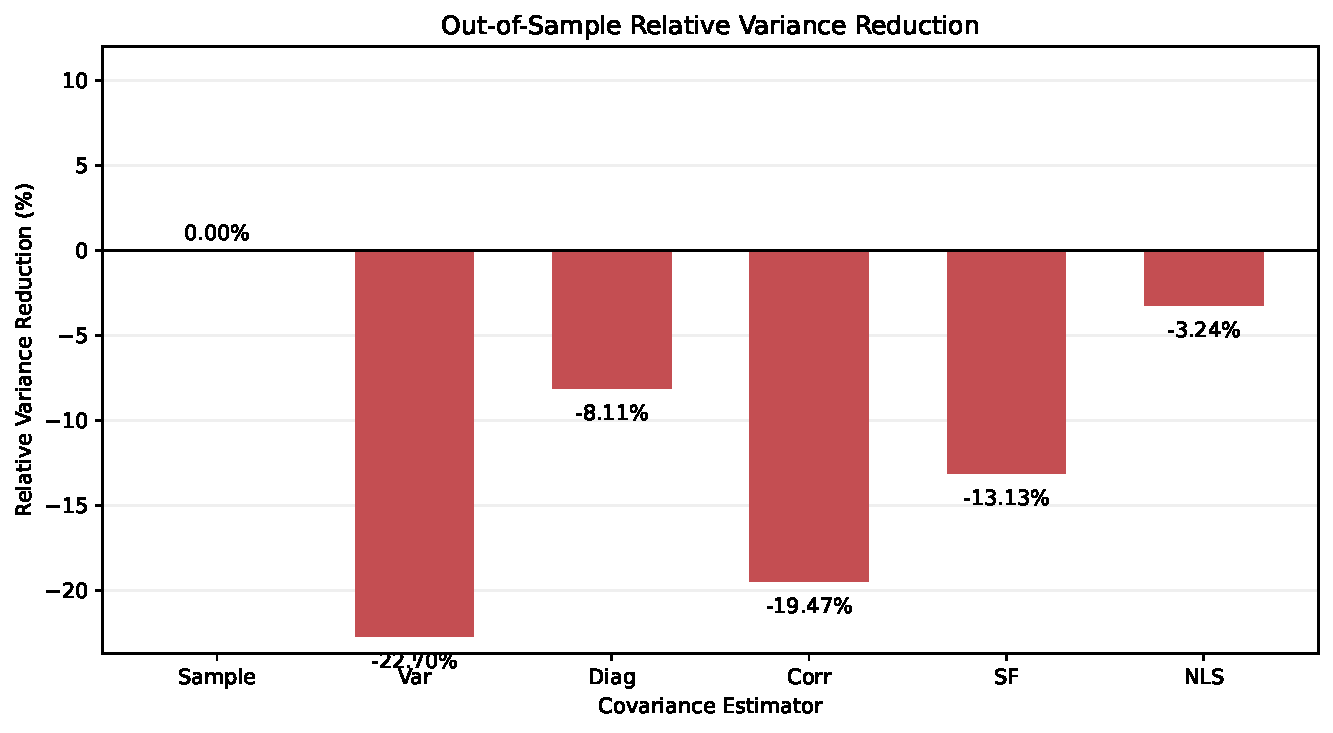
\includegraphics[width=0.3\textwidth]{GMVP_OOS_RVR_low.pdf}
	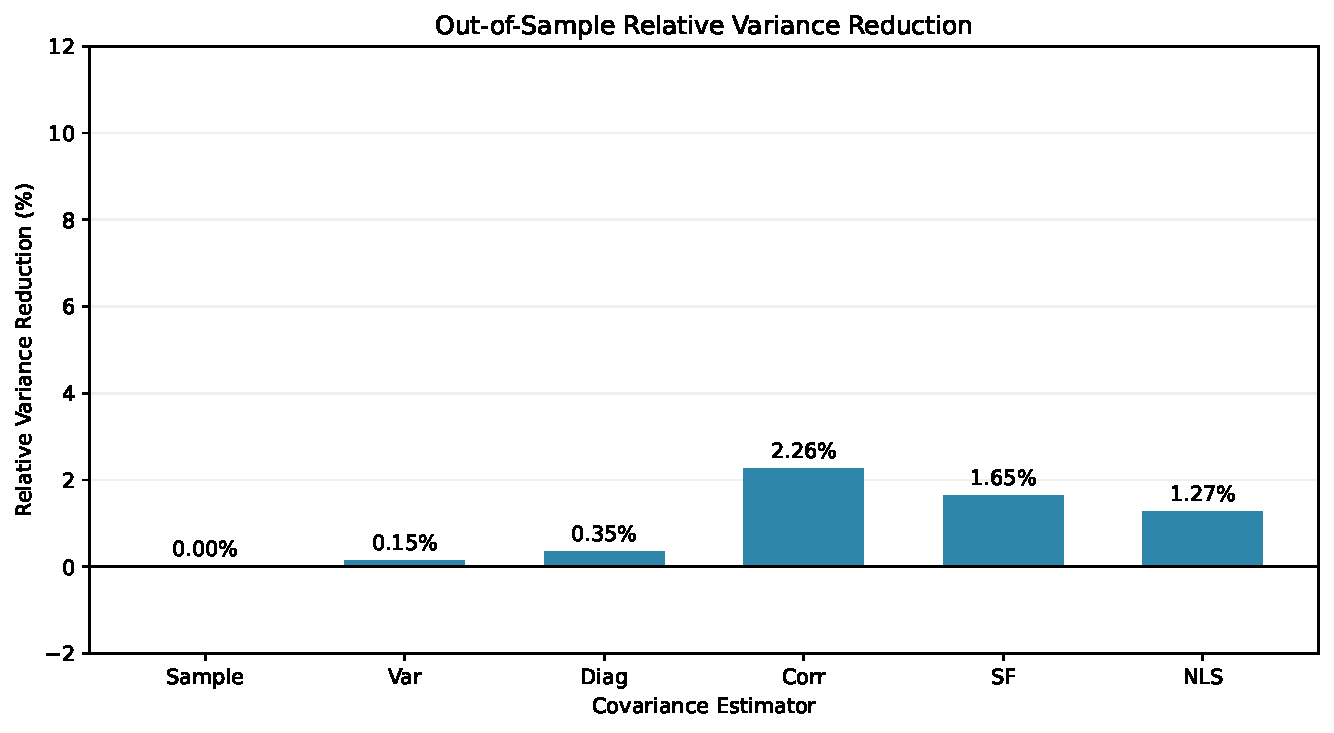
\includegraphics[width=0.3\textwidth]{GMVP_OOS_RVR_medium.pdf}
	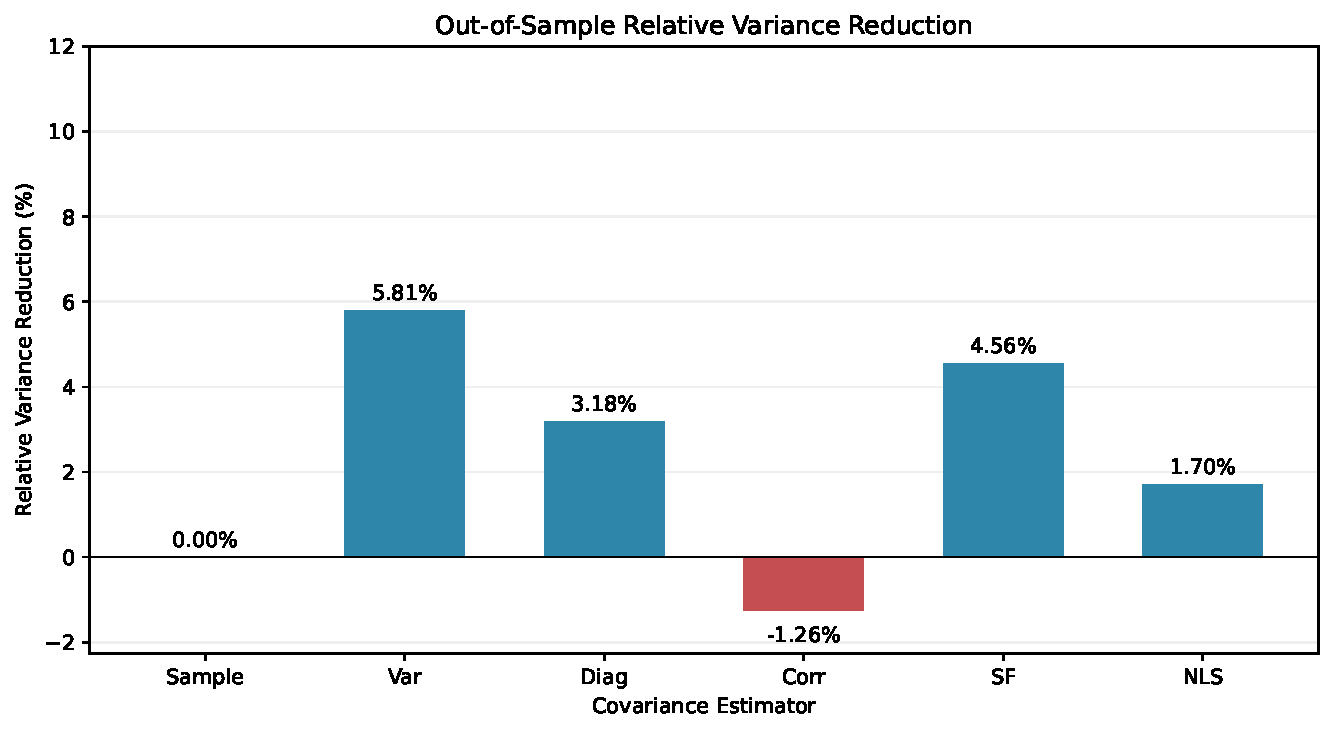
\includegraphics[width=0.3\textwidth]{GMVP_OOS_RVR_high.pdf}
\end{center}


\begin{sidewaystable}[p]
	\centering
	\caption{Robustness results across 150 portfolios}
	\label{tab:robustness_150}
	\scriptsize
	\setlength{\tabcolsep}{4pt}
	\begin{tabular}{llrrrrrrrrrr}
		\hline
		Tier & Method
		& Mean RVR
		& Median RVR
		& Positive RVR
		& Mean Return
		& OOS Variance
		& OOS Volatility
		& Sharpe
		& Turnover
		& HHI
		& HAC $p$ \\
		&
		& (\%) & (\%) & (\%)
		& (monthly) & (monthly)
		& (annual) & (annual)
		& & & \\
		\hline
		High & Var
		& 1.128 & 1.354 & 72
		& 0.01119 & 0.003108 & 0.19220
		& 0.7024 & 0.02638 & 0.2855 & 0.1629 \\
		
		& Diag
		& 0.808 & 0.789 & 82
		& 0.01111 & 0.003121 & 0.19257
		& 0.6966 & 0.02624 & 0.3297 & 0.0203 \\
		
		& Corr
		& 0.651 & 0.911 & 60
		& 0.01098 & 0.003116 & 0.19253
		& 0.6883 & 0.02357 & 0.3530 & 0.3840 \\
		
		& SF
		& 0.530 & 0.453 & 74
		& 0.01100 & 0.003130 & 0.19285
		& 0.6881 & 0.02580 & 0.3410 & 0.2236 \\
		
		& NLS
		& 0.389 & 0.584 & 66
		& 0.01105 & 0.003134 & 0.19298
		& 0.6907 & 0.02657 & 0.3273 & 0.2003 \\
		\hline
		Medium & Var
		& -1.305 & -0.676 & 48
		& 0.00648 & 0.002138 & 0.15909
		& 0.4890 & 0.02622 & 0.2102 & 0.4168 \\
		
		& Diag
		& 0.568 & 0.477 & 68
		& 0.00624 & 0.002093 & 0.15755
		& 0.4756 & 0.02627 & 0.2523 & 0.3231 \\
		
		& Corr
		& 0.547 & 0.593 & 54
		& 0.00571 & 0.002093 & 0.15752
		& 0.4350 & 0.02339 & 0.2673 & 0.3557 \\
		
		& SF
		& 0.670 & 0.905 & 64
		& 0.00563 & 0.002088 & 0.15739
		& 0.4293 & 0.02436 & 0.2627 & 0.1907 \\
		
		& NLS
		& 0.365 & 0.328 & 56
		& 0.00618 & 0.002097 & 0.15770
		& 0.4707 & 0.02677 & 0.2476 & 0.3640 \\
		\hline
		Low & Var
		& -35.018 & -29.789 & 28
		& 0.00831 & 0.002472 & 0.17081
		& 0.5749 & 0.03089 & 0.1210 & 0.0149 \\
		
		& Diag
		& -0.611 & 0.518 & 54
		& 0.00622 & 0.001868 & 0.14921
		& 0.5040 & 0.02503 & 0.1701 & 0.8698 \\
		
		& Corr
		& 0.158 & 0.895 & 64
		& 0.00538 & 0.001859 & 0.14878
		& 0.4396 & 0.02463 & 0.2118 & 0.8593 \\
		
		& SF
		& -1.356 & -0.850 & 42
		& 0.00513 & 0.001883 & 0.14981
		& 0.4150 & 0.02360 & 0.2179 & 0.5334 \\
		
		& NLS
		& 0.986 & 0.950 & 74
		& 0.00582 & 0.001843 & 0.14817
		& 0.4773 & 0.02791 & 0.1996 & 0.1317 \\
		\hline
	\end{tabular}
	
	\vspace{2mm}
	\begin{minipage}{0.95\textwidth}
		\footnotesize
		\textit{Тайлбар:}
		Корреляцийн ангилал бүрд 50 багц хамрагдсан.
		Дундаж болон медиан RVR, эерэг RVR-тэй багцын эзлэх хувийг
		хувиар илэрхийлсэн. Өгөөж болон дисперсийг сарын,
		харин хэлбэлзэл болон Sharpe харьцааг жилийн хэмжээсээр
		тооцсон. HAC шалгуурын $p$-утгууд нь хоёр талт бөгөөд
		олон харьцуулалтын засвар хийгээгүй.
	\end{minipage} 
\end{sidewaystable}

Ковариацын матрицын агшилтын аргуудын үр дүн багцын бүрэлдэхүүн болон хөрөнгүүдийн хоорондын корреляцийн бүтцээс хэрхэн хамаарч байгааг үнэлэх зорилгоор өндөр, дунд, бага корреляцитай ангилал тус бүрээс 50, нийт 150 багцад шинжилгээг давтан гүйцэтгэв. Хүснэгтэд Sample ковариацын матрицыг суурь болгон авч, агшилтын таван аргын OOS дисперсийн бууралт, өгөөж, хэлбэлзэл, Sharpe харьцаа, багцын жингийн тогтвортой байдал болон төвлөрлийн үзүүлэлтүүдийг нэгтгэн харуулав.

Өндөр корреляцитай багцуудын хувьд бүх агшилтын арга эерэг дундаж RVR үзүүлсэн бөгөөд тогтмол дисперсийн зорилтот матрицтай Var арга хамгийн өндөр дундаж дисперсийн бууралттай (1.128\%) байна. Харин Diag арга 50 багцын 82\%-д дисперс бууруулж, хамгийн өндөр эерэг RVR-ийн эзлэх хувьтай гарсан. Түүнчлэн Diag аргын HAC шалгуурын үр дүн (\(p=0.0203\)) нь Sample аргатай харьцуулсан дундаж дисперсийн ялгаа 5\%-ийн түвшинд статистикийн ач холбогдолтой болохыг харуулж байна. Бусад агшилтын аргуудын хувьд статистикийн ач холбогдолтой ялгаа илрээгүй.

Дунд корреляцитай багцуудын хувьд Single--Factor (SF) арга
хамгийн өндөр дундаж RVR (0.670\%) үзүүлсэн бол
Diag (0.568\%) болон Corr (0.547\%) аргууд
ойролцоо үр дүнтэй байна.
Харин Var аргын дундаж RVR сөрөг ($-1.305\%$)
бөгөөд багцуудын 48\%-д дисперс бууруулжээ.
Гэсэн хэдий ч энэ ангилалд бүх аргын HAC шалгуурын
$p$-утга 0.05-аас их байгаа тул Sample аргатай
харьцуулсан дундаж дисперсийн ялгаа статистикийн
ач холбогдолтой гэж үзэх үндэслэлгүй байна.

Бага корреляцитай багцуудын хувьд аргуудын үр дүн илүү
ялгаатай байна. Var арга хамгийн өндөр эрсдэлтэй бөгөөд
дундаж RVR $-35.018\%$, медиан RVR $-29.789\%$ гарч,
багцуудын ердөө 28\%-д дисперс бууруулсан.
HAC шалгуурын үр дүн ($p=0.0149$) нь энэ аргын дисперс
Sample аргатай харьцуулахад өссөн чиглэлтэй статистикийн
ач холбогдолтой ялгааг харуулж байна.
Харин NLS арга хамгийн өндөр дундаж RVR (0.986\%)
үзүүлж, багцуудын 74\%-д дисперс бууруулсан боловч
HAC шалгуурын үр дүн ($p=0.1317$) статистикийн
ач холбогдолгүй байна.

Багцын бусад үзүүлэлтүүдийг авч үзвэл, агшилтын аргуудын OOS хэлбэлзэл, Sharpe харьцаа болон жингийн бүтцэд тодорхой ялгаа ажиглагдсан. Тухайлбал, бага корреляцитай багцуудын Var арга хамгийн бага дундаж HHI (0.121) буюу хөрөнгө оруулалтын жин харьцангуй тархмал бүтэцтэй боловч хамгийн өндөр жилийн OOS хэлбэлзэлтэй (17.081\%) байна. Харин NLS арга энэ ангилалд хамгийн бага жилийн OOS хэлбэлзэлтэй (14.817\%) гарсан. Энэ нь багцын жингийн төвлөрөл бага байх нь заавал эрсдэл бага байх нөхцөл биш болохыг харуулж байна.

Ерөнхийд нь дүгнэвэл, 150 багцын robustness шинжилгээний үр дүн ковариацын матрицын агшилтын аргуудын давуу тал бүх багцад ижил хэмжээгээр илэрдэггүйг харуулж байна. Өндөр корреляцитай багцуудад бүх арга эерэг дундаж дисперсийн бууралт үзүүлсэн бол бага корреляцитай багцуудад аргуудын үр дүн илүү ялгаатай, ялангуяа Var аргын гүйцэтгэл мэдэгдэхүйц сул байна. HAC шалгуураар 15 харьцуулалтын зөвхөн хоёрт нь 5\%-ийн түвшинд статистикийн ач холбогдол илэрсэн бөгөөд эдгээр \(p\)-утгад олон харьцуулалтын засвар хийгээгүй тул үр дүнг болгоомжтой тайлбарлах шаардлагатай. Иймээс бага \(N/T\) нөхцөлд ковариацын матрицын агшилт нь Sample аргатай харьцуулахад OOS дисперсийг тогтвортой бууруулдаг гэсэн ерөнхий дүгнэлт хийх боломжгүй бөгөөд түүний үр нөлөө багцын корреляцийн бүтэц болон сонгосон агшилтын аргаас хамаарч байгааг энэхүү шинжилгээ харуулж байна.

% Preamble:
% \usepackage{rotating}
% \usepackage{graphicx}
% \usepackage{booktabs}

\begin{sidewaystable}[p]
	\centering
	\caption{Нэмэлтээр сонгосон багцуудын OOS гүйцэтгэлийн харьцуулалт}
	\label{tab:additional_portfolios}
	\tiny
	\setlength{\tabcolsep}{3pt}
	\renewcommand{\arraystretch}{1.12}
	
	\resizebox{\textheight}{!}{%
		\begin{tabular}{llrrrrrrrrp{7.3cm}}
			\toprule
			Selection & Estimator & Mean & RVR & Monthly & Monthly
			& Sharpe & Turnover & HHI & HAC & Tickers \\
			Target & & Corr. & (\%) & Return (\%) & Volatility (\%)
			& & & & $p$-value & \\
			\midrule
			
			All & Sample & 0.3073 & 0.000 & 1.103 & 3.850 & 0.993 & 0.0292 & 0.2043 & -- & BA, BMY, COST, DHI, FTI, IBM, NKE, RF, SCHW, VRSN \\
			& $Var^{*}$ & 0.3073 & 4.952 & 1.046 & 3.753 & 0.965 & 0.0274 & 0.1867 & 0.0331 & \\
			& Diag & 0.3073 & 3.217 & 1.073 & 3.787 & 0.981 & 0.0279 & 0.1966 & 0.0436 & \\
			& Corr & 0.3073 & 3.600 & 1.049 & 3.780 & 0.962 & 0.0278 & 0.2046 & 0.6070 & \\
			& SF & 0.3073 & 4.019 & 1.111 & 3.772 & 1.020 & 0.0273 & 0.2033 & 0.1884 & \\
			& NLS & 0.3073 & 4.540 & 1.041 & 3.761 & 0.959 & 0.0269 & 0.1939 & 0.0607 & \\
			\midrule
			
			Var & Sample & 0.3073 & 0.000 & 1.103 & 3.850 & 0.993 & 0.0292 & 0.2043 & -- & BA, BMY, COST, DHI, FTI, IBM, NKE, RF, SCHW, VRSN \\
			& $Var^{*}$ & 0.3073 & 4.952 & 1.046 & 3.753 & 0.965 & 0.0274 & 0.1867 & 0.0331 & \\
			& Diag & 0.3073 & 3.217 & 1.073 & 3.787 & 0.981 & 0.0279 & 0.1966 & 0.0436 & \\
			& Corr & 0.3073 & 3.600 & 1.049 & 3.780 & 0.962 & 0.0278 & 0.2046 & 0.6070 & \\
			& SF & 0.3073 & 4.019 & 1.111 & 3.772 & 1.020 & 0.0273 & 0.2033 & 0.1884 & \\
			& NLS & 0.3073 & 4.540 & 1.041 & 3.761 & 0.959 & 0.0269 & 0.1939 & 0.0607 & \\
			\midrule
			
			Diag & Sample & 0.2432 & 0.000 & 0.141 & 3.998 & 0.122 & 0.0268 & 0.2376 & -- & ADBE, AN, CTAS, ES, GME, MAS, NTAP, SRE, SYY, TAP \\
			& Var & 0.2432 & -12.701 & 0.217 & 4.244 & 0.177 & 0.0287 & 0.1000 & 0.5644 & \\
			& Diag & 0.2432 & 0.613 & 0.141 & 3.985 & 0.122 & 0.0244 & 0.1402 & 0.9673 & \\
			& Corr & 0.2432 & -0.107 & 0.145 & 4.000 & 0.126 & 0.0274 & 0.2339 & 0.9560 & \\
			& SF & 0.2432 & -8.020 & 0.182 & 4.155 & 0.151 & 0.0211 & 0.2763 & 0.3830 & \\
			& NLS & 0.2432 & 0.794 & 0.078 & 3.982 & 0.068 & 0.0273 & 0.2175 & 0.8468 & \\
			\midrule
			
			Corr & Sample & 0.2335 & 0.000 & 0.308 & 4.368 & 0.244 & 0.0382 & 0.2082 & -- & BDX, DRI, EFX, GPC, HRB, HRL, HSY, INTC, ORLY, TRIP \\
			& Var & 0.2335 & 8.632 & 0.329 & 4.175 & 0.273 & 0.0373 & 0.1681 & 0.1223 & \\
			& Diag & 0.2335 & 4.858 & 0.245 & 4.261 & 0.199 & 0.0372 & 0.1879 & 0.2307 & \\
			& Corr & 0.2335 & -5.166 & 0.031 & 4.480 & 0.024 & 0.0320 & 0.1866 & 0.7313 & \\
			& SF & 0.2335 & 4.791 & 0.011 & 4.262 & 0.009 & 0.0313 & 0.1954 & 0.6546 & \\
			& $NLS^{*}$ & 0.2335 & 5.657 & 0.337 & 4.243 & 0.275 & 0.0381 & 0.1868 & 0.0124 & \\
			\midrule
			
			SF & Sample & 0.2092 & 0.000 & 0.407 & 4.242 & 0.332 & 0.0348 & 0.2048 & -- & ADBE, ED, GME, HSY, LMT, MCHP, PFG, PH, WDC, WMT \\
			& $Var^{*}$ & 0.2092 & -51.840 & 1.654 & 5.227 & 1.096 & 0.0350 & 0.1000 & 0.0334 & \\
			& Diag & 0.2092 & 3.220 & 0.937 & 4.173 & 0.778 & 0.0286 & 0.1443 & 0.7040 & \\
			& Corr & 0.2092 & 1.976 & 0.469 & 4.200 & 0.387 & 0.0321 & 0.2061 & 0.0659 & \\
			& SF & 0.2092 & -17.000 & 0.657 & 4.588 & 0.496 & 0.0246 & 0.2540 & 0.3028 & \\
			& NLS & 0.2092 & -0.006 & 0.411 & 4.242 & 0.336 & 0.0326 & 0.1981 & 0.9973 & \\
			\midrule
			
			NLS & Sample & 0.2723 & 0.000 & -0.215 & 4.745 & -0.157 & 0.0433 & 0.2195 & -- & BKNG, COF, COST, HRL, HUM, KIM, NKE, ORCL, PHM, UNH \\
			& Var & 0.2723 & 2.490 & -0.187 & 4.686 & -0.138 & 0.0394 & 0.1832 & 0.4114 & \\
			& Diag & 0.2723 & 3.958 & -0.226 & 4.650 & -0.168 & 0.0395 & 0.2024 & 0.1352 & \\
			& Corr & 0.2723 & 11.084 & -0.329 & 4.475 & -0.255 & 0.0352 & 0.2043 & 0.1833 & \\
			& SF & 0.2723 & 2.404 & -0.397 & 4.688 & -0.293 & 0.0377 & 0.2143 & 0.4767 & \\
			& NLS & 0.2723 & 1.137 & -0.280 & 4.718 & -0.206 & 0.0414 & 0.1976 & 0.5294 & \\
			\bottomrule
		\end{tabular}%
	}
	
	\vspace{3mm}
	\begin{minipage}{0.96\textheight}
		\footnotesize
		\textit{Тайлбар:}
		Selection Target нь validation хугацаанд багцыг сонгоход
		ашигласан зорилтот шалгуур юм. All шалгуур нь таван
		агшилтын аргын хамгийн бага RVR-ийг хамгийн өндөр
		болгох, бусад шалгуур нь харгалзах аргын RVR-ийг
		хамгийн өндөр болгоход чиглэсэн.
		
		All болон Var шалгуураар ижил 10 хувьцааны багц
		сонгогдсон тул эдгээрийн OOS үр дүн давхцаж байна.
		Tickers баганад тухайн багцын хувьцааны кодыг
		нэг удаа харуулав.
		
		Бүх багцад $N=10$, $T=120$, $N/T=0.0833$.
		Mean Corr. нь сургалтын хугацааны дундаж хос
		корреляци юм. RVR нь Sample аргатай харьцуулсан
		OOS дисперсийн бууралтын хувь бөгөөд эерэг утга
		нь дисперс буурсныг, сөрөг утга нь өссөнийг илэрхийлнэ.
		
		Өгөөж болон хэлбэлзлийг сарын хувиар,
		Sharpe харьцааг жилийн хэмжээсээр илэрхийлсэн.
		Turnover нь нэг талын багцын эргэлт,
		HHI нь багцын төвлөрлийн үзүүлэлт юм.
		
		HAC $p$-value нь төвлөрүүлсэн квадрат өгөөжийн
		ялгаанд суурилсан, Newey--West стандарт алдаатай
		($L=3$) хоёр талт шалгуурын утга юм.
		Sample нь харьцуулах суурь арга тул
		$p$-value тооцоогүй.
	\end{minipage}
	
\end{sidewaystable}

\noindent
\textbf{All шалгуураар сонгосон багцын хувьд}
бүх агшилтын арга Sample аргатай харьцуулахад OOS дисперсийг
бууруулсан байна. Эдгээрээс Var арга хамгийн өндөр RVR
(4.952\%) үзүүлж, сарын хэлбэлзлийг 3.850\%-аас 3.753\%
болгон бууруулсан бөгөөд HAC шалгуурын үр дүн
(\(p=0.0331\)) нь энэхүү ялгаа 5\%-ийн түвшинд
статистикийн ач холбогдолтойг харуулж байна.
Diag арга мөн дисперсийг 3.217\%-иар бууруулсан бөгөөд
статистикийн ач холбогдолтой (\(p=0.0436\)) байна.
Харин Corr, SF болон NLS аргуудын RVR эерэг боловч
статистикийн ач холбогдолгүй байна.
Иймээс All багцад \textbf{Var арга дисперсийн бууралт
	болон HAC шалгуурын үр дүнгээр хамгийн давуу} байна.

\par\medskip
\noindent
\textbf{Var шалгуураар сонгосон багцын хувьд}
All шалгуураар сонгосон багцтай ижил 10 хувьцаа
сонгогдсон тул OOS гүйцэтгэлийн бүх үзүүлэлт
давхцаж байна. Тухайлбал, Var арга хамгийн өндөр
RVR (4.952\%) үзүүлж, статистикийн ач холбогдолтой
(\(p=0.0331\)) байна. Иймээс Var шалгуураар сонгосон
багцад мөн Var арга хамгийн сайн үр дүн үзүүлсэн
боловч энэ нь All багцаас тусдаа, бие даасан
үр дүн биш юм.

\par\medskip
\noindent
\textbf{Diag шалгуураар сонгосон багцын хувьд}
NLS арга хамгийн өндөр RVR (0.794\%) үзүүлсэн
боловч HAC шалгуураар статистикийн ач холбогдолгүй
(\(p=0.8468\)) байна. Diag аргын RVR 0.613\% бөгөөд
мөн статистикийн ач холбогдолгүй (\(p=0.9673\)) байна.
Харин Var, Corr болон SF аргуудын RVR сөрөг гарсан
нь Sample аргатай харьцуулахад OOS дисперс өссөнийг
илэрхийлнэ. Гэвч эдгээр өсөлт ч статистикийн
ач холбогдолгүй байна.
Иймээс Diag багцад \textbf{Sample аргаас статистикийн
	ач холбогдолтойгоор бага дисперстэй агшилтын арга
	илрээгүй} бөгөөд тухайн багцад аль нэг агшилтын
аргыг давуу гэж сонгох статистикийн үндэслэл
тогтоогдсонгүй.

\par\medskip
\noindent
\textbf{Corr шалгуураар сонгосон багцын хувьд}
Var арга хамгийн өндөр RVR (8.632\%) үзүүлсэн
боловч HAC шалгуурын үр дүн (\(p=0.1223\))
статистикийн ач холбогдолгүй байна.
Харин NLS арга 5.657\%-ийн дисперсийн бууралт
үзүүлсэн бөгөөд HAC шалгуураар статистикийн
ач холбогдолтой (\(p=0.0124\)) байна.
Үүний эсрэгээр Corr аргын RVR $-5.166\%$ гарч,
OOS дисперс Sample аргатай харьцуулахад өссөн
боловч ялгаа статистикийн ач холбогдолгүй
(\(p=0.7313\)) байна.
Иймээс Corr багцад \textbf{NLS арга статистикийн
	ач холбогдолтой дисперсийн бууралт үзүүлсэн
	цорын ганц агшилтын арга} бөгөөд Corr аргын
хувьд дисперсийн бууралтын давуу тал
ажиглагдсангүй.

\par\medskip
\noindent
\textbf{SF шалгуураар сонгосон багцын хувьд}
Diag арга хамгийн өндөр эерэг RVR (3.220\%)
үзүүлсэн боловч статистикийн ач холбогдолгүй
(\(p=0.7040\)) байна.
Corr арга мөн дисперсийг 1.976\%-иар бууруулсан
боловч HAC шалгуурын үр дүн (\(p=0.0659\))
нь 5\%-ийн түвшинд статистикийн ач холбогдолгүй
байна.
Харин Var арга хамгийн их дисперсийн өсөлттэй
(RVR $-51.840\%$) бөгөөд энэ ялгаа статистикийн
ач холбогдолтой (\(p=0.0334\)) байна.
SF аргын RVR $-17.000\%$ гарсан боловч
статистикийн ач холбогдолгүй (\(p=0.3028\)) байна.
Иймээс SF багцад \textbf{Sample аргаас статистикийн
	ач холбогдолтойгоор бага дисперстэй агшилтын арга
	илрээгүй}, харин Var арга статистикийн
ач холбогдолтойгоор өндөр дисперстэй байна.

\par\medskip
\noindent
\textbf{NLS шалгуураар сонгосон багцын хувьд}
бүх агшилтын арга Sample аргатай харьцуулахад
OOS дисперсийг бууруулсан байна.
Эдгээрээс Corr арга хамгийн өндөр RVR (11.084\%)
үзүүлж, сарын хэлбэлзлийг 4.745\%-аас 4.475\%
болгон бууруулсан.
Харин NLS аргын RVR 1.137\% байна.
Гэсэн хэдий ч бүх аргын HAC шалгуурын
\(p\)-утга 0.05-аас их байгаа тул дисперсийн
бууралтууд статистикийн ач холбогдолгүй байна.
Иймээс NLS багцад \textbf{Corr арга тоон үзүүлэлтээр
	хамгийн өндөр дисперсийн бууралт үзүүлсэн боловч
	статистикийн ач холбогдолтой давуу тал
	тогтоогдсонгүй}.

\par\medskip
\noindent
\textbf{Нийт үр дүнгээс харахад},
All болон Var шалгуураар сонгосон ижил багцад
Var арга, Corr шалгуураар сонгосон багцад NLS арга
Sample аргатай харьцуулахад статистикийн
ач холбогдолтой дисперсийн бууралт үзүүлсэн байна.
Харин Diag, SF болон NLS шалгуураар сонгосон
багцуудад Sample аргаас статистикийн ач
холбогдолтойгоор бага дисперстэй агшилтын
арга илрээгүй.

Түүнчлэн SF шалгуураар сонгосон багцад Var аргын
RVR $-51.840\%$ гарч, Sample аргатай харьцуулахад
OOS дисперс өссөн бөгөөд HAC шалгуурын үр дүн
(\(p=0.0334\)) нь энэхүү өсөлт 5\%-ийн түвшинд
статистикийн ач холбогдолтойг харуулж байна.

Иймээс нэмэлт шинжилгээнд агшилтын аргуудын
OOS дисперсийн бууралт багцын сонголтоос
хамааран ялгаатай гарсан бөгөөд бүх багцад
тогтвортой давуу тал үзүүлсэн нэг арга
тогтоогдсонгүй.

% Preamble:
% \usepackage{booktabs}

\begin{table}[htbp]
	\centering
	\caption{Статистикийн ач холбогдолтой OOS дисперсийн
		ялгаа үзүүлсэн багцуудын хөрөнгө оруулалтын жин}
	\label{tab:significant_portfolio_weights}
	\small
	\setlength{\tabcolsep}{9pt}
	\renewcommand{\arraystretch}{1.1}
	
	\begin{tabular}{lrrr}
		\toprule
		Ticker & All/Var--Var & Corr--NLS & SF--Var \\
		\midrule
		ADBE & -- & -- & 10.00 \\
		BA   & 0.00 & -- & -- \\
		BDX  & -- & 18.80 & -- \\
		BMY  & 24.47 & -- & -- \\
		COST & 23.82 & -- & -- \\
		DHI  & 0.00 & -- & -- \\
		DRI  & -- & 2.23 & -- \\
		ED   & -- & -- & 10.00 \\
		EFX  & -- & 0.00 & -- \\
		FTI  & 0.00 & -- & -- \\
		GME  & -- & -- & 10.00 \\
		GPC  & -- & 0.00 & -- \\
		HRB  & -- & 13.18 & -- \\
		HRL  & -- & 22.58 & -- \\
		HSY  & -- & 26.24 & 10.00 \\
		IBM  & 11.66 & -- & -- \\
		INTC & -- & 6.10 & -- \\
		LMT  & -- & -- & 10.00 \\
		MCHP & -- & -- & 10.00 \\
		NKE  & 7.55 & -- & -- \\
		ORLY & -- & 7.11 & -- \\
		PFG  & -- & -- & 10.00 \\
		PH   & -- & -- & 10.00 \\
		RF   & 0.00 & -- & -- \\
		SCHW & 13.15 & -- & -- \\
		TRIP & -- & 3.76 & -- \\
		VRSN & 19.35 & -- & -- \\
		WDC  & -- & -- & 10.00 \\
		WMT  & -- & -- & 10.00 \\
		\midrule
		\textbf{Total (\%)} & \textbf{100.00} & \textbf{100.00}
		& \textbf{100.00} \\
		\midrule
		RVR (\%) & 4.952 & 5.657 & -51.840 \\
		HAC $p$-value & 0.0331 & 0.0124 & 0.0334 \\
		\bottomrule
	\end{tabular}
	
	\vspace{2mm}
	\begin{minipage}{0.95\linewidth}
		\footnotesize
		\textit{Тайлбар:}
		Багцын жинг хувиар илэрхийлэв.
		-- тэмдэглэгээ нь тухайн хувьцаа багцад
		сонгогдоогүй, 0.00 нь сонгогдсон боловч
		тэг жинтэй байгааг илэрхийлнэ.
		Жингийн нийлбэрийг 100.00\% болгохын тулд
		тоймлолтын зөрүүг сүүлийн сонгосон
		хувьцааны жинд тохируулсан.
		
		All болон Var шалгуураар ижил 10 хувьцааны
		багц сонгогдсон тул тэдгээрийн Var аргын
		жинг нэг баганад харуулав.
		
		All/Var--Var болон Corr--NLS аргууд
		статистикийн ач холбогдолтой OOS дисперсийн
		бууралт үзүүлсэн бол SF--Var арга
		статистикийн ач холбогдолтой дисперсийн
		өсөлт үзүүлсэн.
		
		HAC $p$-утгууд нь олон харьцуулалтын
		засвар хийгдээгүй хоёр талт шалгуурын
		үр дүн юм.
	\end{minipage}
	
\end{table}

Хүснэгт~\ref{tab:significant_portfolio_weights}-д
OOS дисперсийн ялгаа нь статистикийн ач холбогдолтой
гарсан гурван үр дүнгийн багцын жингийн бүтцийг
харуулав. All болон Var шалгуураар ижил багц
сонгогдсон тул тэдгээрийн Var аргын жинг нэгтгэн
үзүүлсэн.

All/Var багцын хувьд Var аргаар тооцсон жин
BMY (24.47\%), COST (23.82\%), VRSN (19.35\%),
SCHW (13.15\%) болон IBM (11.66\%) хувьцаанд
голчлон төвлөрсөн байна. Харин BA, DHI, FTI
болон RF хувьцааны жин тэг гарсан.
Энэ багцад Var арга Sample аргатай харьцуулахад
OOS дисперсийг 4.952\%-иар бууруулсан бөгөөд
ялгаа статистикийн ач холбогдолтой
(\(p=0.0331\)) байна.

Corr шалгуураар сонгосон багцын хувьд
NLS аргаар тооцсон жин HSY (26.24\%),
HRL (22.58\%), BDX (18.80\%) болон
HRB (13.18\%) хувьцаанд харьцангуй
өндөр төвлөрсөн байна.
Харин EFX болон GPC хувьцааны жин тэг гарсан.
Энэ багцад NLS арга OOS дисперсийг
5.657\%-иар бууруулж, статистикийн
ач холбогдолтой үр дүн үзүүлсэн
(\(p=0.0124\)) байна.

SF шалгуураар сонгосон багцын хувьд
Var аргаар тооцсон жин бүх 10 хувьцаанд
ижил буюу 10.00\% байна.
Ингэснээр тэнцүү жинтэй багц үүссэн боловч
Sample аргатай харьцуулахад OOS дисперс
51.840\%-иар өссөн бөгөөд энэхүү өсөлт
статистикийн ач холбогдолтой
(\(p=0.0334\)) байна.

Эдгээр үр дүнгээс харахад статистикийн
ач холбогдолтой дисперсийн бууралт үзүүлсэн
All/Var--Var болон Corr--NLS багцуудын жин
тодорхой хувьцаанд төвлөрсөн байхад,
дисперсийн өсөлт үзүүлсэн SF--Var багцын
жин тэнцүү хуваарилагдсан байна.
Гэхдээ энэхүү ялгаа нь багцын жингийн
төвлөрөл дангаараа OOS дисперсийн
өөрчлөлтийг тодорхойлдог гэсэн үг биш юм.